
\documentclass{article}

%-------------------------------------------------------------------------------------------------------------
%  package
%--------------------------------------------------------------------------------------------------------------
%版面規劃(a4大小,上下左右距0.9inch)
\usepackage[a4paper,margin=0.9in]{geometry}
%作者資訊
\usepackage{authblk}
%中文化package
\usepackage{CJKutf8}

%分兩欄
\usepackage{multicol}
%分欄之後上圖需要有的package
\usepackage{float}
%然後若是需要在其中一欄上面加圖片=>[H大寫]
%要跨欄橫幅的圖片=>{figure*星號要加}[htbp]


%和插入圖片相關的package
\usepackage{graphicx}
\usepackage[tight]{subfigure}
\subfiguretopcaptrue
\usepackage{amsmath,booktabs,threeparttable,url, bm}
%\usepackage[hyphenbreaks]{breakurl}


%連結註腳網頁
\usepackage[colorlinks,linkcolor=blue]{hyperref}


%\newcommand{\cntext}{\begin{CJK}{UTF8}{bsmi}\end{CJK}}

\title{Assignment 7 of Computational Astrophysics in NTHU}
\author{Wei-Hsiang Yu 游惟翔}
\affil{Department of Physics, National Tsing Hua University, Hsinchu, Taiwan}

%-------------------------------------------------------------------------------------------------------------
%  文件開始
%--------------------------------------------------------------------------------------------------------------
\begin{document}

\begin{CJK}{UTF8}{bsmi}
%中文化需要加上此行才有title/author/date
\maketitle
\end{CJK}


%-------------------------------------------------------------------------------------------------------------
%  Written Assignments
%--------------------------------------------------------------------------------------------------------------
\section{Written Assignments}
\subsection*{Q1 : Stellar structure - polytrope.}
\subsubsection*{Q1.a. : polytropic constant $K$}
\begin{equation}
    K=\begin{bmatrix}
        \frac{4\pi}{\xi^{n+1}(-\theta'_n)^{n-1}}
        \end{bmatrix}_{\xi_1}^{\frac{1}{n}}
      \frac{G}{n+1}M^{1-\frac{1}{n}}R^{-1+\frac{3}{n}}
      \label{eq:K}
\end{equation}

\subsubsection*{Q1.b. : central pressure $P_c$}
\begin{equation}
    P_{c}=\frac{8.952\times10^{14}}{(n+1)(\theta'_n)^2_{\xi_{1}}}
          (\frac{M}{M_{\odot}})^2(\frac{R}{R_{\odot}})^{-4}[dyne\ cm^{-2}]
    \label{eq:Pc}
\end{equation}

\subsubsection*{Q1.c. : central temperature $T_c$}
\begin{equation}
    T_c=\frac{2.293\times10^7}{(n+1)(-\xi\theta'_n)_{\xi_1}}\mu 
         (\frac{M}{M_{\odot}})(\frac{R}{R_{\odot}})^{-1}[K]
    \label{eq:Tc}
\end{equation}

\hrulefill % 實線
\subsubsection*{Derivation}

From the lecture in the class, we have derived the \textbf{Lane-Emden equation} :\\
\begin{equation}
    \frac{(n+1)P_c}{4\pi G\rho_c^2}
    \frac{1}{r}\frac{d}{dr}
    (r^2\frac{d\theta}{dr})+\theta^n
    =
    \frac{1}{\xi^2}\frac{d}{d\epsilon }(\epsilon^2\frac{d\theta_n}{d\xi})
    +\theta_n^n=0
    \label{eq:L-E}
\end{equation}
We also define a new \textbf{dimensionless radial coordinate} $\xi$ and have Eq.\ref{eq:rn} and applied it to Eq.\ref{eq:L-E} later part.\\
\begin{equation}
    r=r_n\xi
    \mbox{ where we define }
    r_n^2=\frac{(n+1)P_c}{4\pi G\rho_c^2}
    \label{eq:r}
\end{equation}
And we also have \textbf{the power law for pressure}:
\begin{equation}
    P(r)=K\rho_c ^{1+\frac{1}{n}}\theta^{1+\frac{1}{n}}(r)
    =P_c\ \theta^{1+\frac{1}{n}}(r)
    \label{eq:P}
\end{equation}

Based on those information, we and find $K$ when apply Pc in Eq.\ref{eq:P} to Eq.\ref{eq:r}
\begin{equation}
    r_n^2=\frac{(n+1)P_c}{4\pi G\rho_c^2}
    =\frac{(n+1)K\rho_c^{1+\frac{1}{n}}}{4\pi G\rho_c^2}
    =\frac{(n+1)K\rho_c^{\frac{1}{n}-1}}{4\pi G}
    \label{eq:rn}
\end{equation}

And then we can consider another aspect - mass (implied by Eq.\ref{eq:K} have M component), use the mass conservation mention in the lecture.
\begin{equation*}
    dM_r=4\pi r^2 \rho dr
\end{equation*}

Then do integral and use the dimensionless radial coordinate Eq.\ref{eq:r} ($r=r_n\xi$ , $R=r_n\xi_1$ , $\rho=\rho_c\theta_n^n$)
$$
M=\int_{0}^{R}4\pi r^2 \rho dr
=4\pi r_n^3\rho_c\int_{0}^{\xi_1}\xi^2\theta_n^nd\xi
$$

Recall \textbf{Lane-Emden equation}(Eq.\ref{eq:L-E}) : $\frac{d}{d\epsilon }(\xi^2\frac{d\theta_n}{d\xi})=-\xi^2\theta_n^n$ and can change variable for the integral.

\begin{equation}
M=-4\pi r_n^3\rho_c\int_{0}^{\xi_1}d(\xi^2 \frac{d\theta_n}{d\xi})
=-4\pi r_n^3\rho_c\xi_1^2 \frac{d\theta_n}{d\xi}|_{\xi_1}
=-4\pi r_n^3\rho_c\xi_1^2 \theta_n'|_{\xi_1}
    \label{eq:M}
\end{equation}

By Eq.\ref{eq:r}, we can get $R=r_n\xi_1$, and substitute it into Eq.\ref{eq:rn} we can get $K$ to the left side of the equation:
\begin{equation}
    \frac{R^2}{\xi_1^2}=\frac{(n+1)K \rho_c^{\frac{1}{n}-1}}{4\pi G}
    \Rightarrow K=\frac{4\pi G R^2}{(n+1)\xi_1^2}\rho_c^{1-\frac{1}{n}}
    \label{eq:kp}
\end{equation}



And then use Eq.\ref{eq:M} to get $\rho^{1-\frac{1}{n}}$ and substitute to the equation:
$$
\rho_c^{1-\frac{1}{n}}=\frac{M}{4\pi r_n^3 \xi_1^2 \theta_n'}|_{\xi_1}^{1-\frac{1}{n}}
$$

After arrange the substitution and we can get the polytropic constant K (Eq.\ref{eq:K})
$$
K=\begin{bmatrix}
        \frac{4\pi}{\xi^{n+1}(-\theta'_n)^{n-1}}
        \end{bmatrix}_{\xi_1}^{\frac{1}{n}}
      \frac{G}{n+1}M^{1-\frac{1}{n}}R^{-1+\frac{3}{n}}
$$

\hrulefill % 實線
\\
And we recall the derivation above,

$$P_c=K \rho_c ^{1+\frac{1}{n}} \mbox{ in Eq.\ref{eq:P}}$$
$$K= \frac{4\pi G R^2}{(n+1)\xi_1^2}\rho_c^{1-\frac{1}{n}} \mbox{ in Eq.\ref{eq:kp}}$$

So we need to get $\rho_c$ and substitute it to let the form of $P_c$ become Eq.\ref{eq:Pc}.
From Eq.\ref{eq:M}, we have the relation between mass and density : $M=-4\pi r_n^3\rho_c\xi_1^2\theta_n'$ and can get $\rho_c$:

\begin{equation}
    \rho_c=-\frac{M}{4\pi r_n^3\xi_1^2(\theta_n')_{\xi_1}}
    \label{eq:rho}
\end{equation}

After substituting, we can get the form of Eq.\ref{eq:Pc}:
$$
    P_c=\frac{4\pi G R^2}{(n+1)\xi_1^2}\rho_c^{1-\frac{1}{n}}\rho_c^{1+\frac{1}{n}}
    =\frac{4\pi G R^2}{(n+1)\xi_1^2}(\frac{M}{4\pi r_n^3\xi_1^2(\theta_n')_{\xi_1}})^2
    =\frac{G/4\pi}{(n+1)(\theta_n')_{\xi_1}^2}M^2R^{-4}
$$

\hrulefill % 實線
\\
Ideal gas EoS:
\begin{equation}
    P=\frac{\rho N_A k T}{\mu}
\end{equation}

we can write:
\begin{equation}
    T_c=K\rho_c ^{\frac{1}{n}}(\frac{\mu}{N_A k})
\end{equation}

and substitute $\rho_c$(Eq.\ref{eq:rho}) and $K$(Eq.\ref{eq:kp}) we have get before, we can get the form of Eq.\ref{eq:Tc}:

$$
T_c
=\frac{4\pi G R^2}{(n+1)\xi_1^2}\rho_c^{1-\frac{1}{n}}\rho_c^{\frac{1}{n}}(\frac{\mu}{N_A k})
=\frac{4\pi G R^2}{(n+1)\xi_1^2}(-\frac{M}{4\pi r_n^3\xi_1^2(\theta_n')_{\xi_1}})(\frac{\mu}{N_A k})
$$


$$
\Rightarrow T_c=-\frac{G/N_A k}{(n+1)(\xi\theta_n')_{\xi_{1}}}\mu MR^{-1}
$$

\subsection*{Q2 : Stellar structure - main-sequence stars.}
Now consider a main-sequence star: $1M_{\odot}=1.989E30(kg)$, $1R_{\odot}=6.9634E8(m) $ with polytrope n=3.

Calculate the central density $\rho_c$, central pressure $P_c$, and central temperature $T_c$. They can be gotten by the equation we have derived before, which is Eq.\ref{eq:rho}, Eq.\ref{eq:Pc} and Eq.\ref{eq:Tc}.
Noted that Eq.\ref{eq:rho} can be substitute by the dimensionless radial coordinate we have defined: $R=r_n\xi_1$.

\textbf{central density} $\rho_c$
$$
\rho_c=-\frac{M\xi_1}{4\pi R^3 (\theta_n')_{\xi_1}}
$$

I use the code we build on class to calculate the value of $\xi_1=6.896$, $\theta_n'=-0.04243$ (from Fig.\ref{fig:pro2})

% %-------------------------------
\begin{figure}
    \centering 
	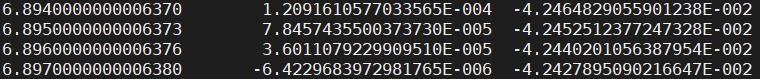
\includegraphics[scale=0.45]{pro2.jpg}
	\caption{calculate the value of $\xi_1$, $\theta_n'$.} %圖片註解
	\label{fig:pro2} %label 用這個就可以引用文章當中
\end{figure}

$$
\rho_c=-
\frac{ 1.989\times10^{30} \times 6.896}
{4\pi \times (6.9634 \times 10^8)^3 \times -0.04243}
= 7.619 \times 10^4
$$

$$
P_c=
\frac{8.952 \times 10^{14}}
{(3+1)(-0.04243)^2}
=1.243 \times 10^{17}
[dyne\ cm^{-2}]
=1.243 \times 10^{11}  [bar]
$$

And from the Sun Fact Sheet provided by the NASA \cite{b1}, $\rho_c=1.622 \times 10^5$, 
$P_c=2.477 \times 10^{11} bar$, which say that we calculate almost half of the truth value of density and pressure.

For Eq.\ref{eq:Tc}, we should first know how to calculate the mean molecular weight $\mu$ \cite{b2}

First we consider the number density of particles,
$$
n=\frac{\rho}{\mu m}
\Rightarrow
\frac{1}{\mu}=\frac{mn}{\rho}
$$

Then this star has a uniform composition X=0.75(H), Y=0.25(He).
$$
X=\frac{m_H n_H}{\rho},
Y=\frac{m_{He} n_{He}}{\rho}
$$

Supposed that the star is fully ionized, so there will be three types of particles in this stars: electron, hydrogen, helium ($n=n_{e^-}+n_H+n_{He}$)
$$
\frac{1}{\mu}=
\frac{m_H n_e}{\rho}+\frac{m_H n_H}{\rho}+\frac{m_{H} n_{He}}{\rho}
$$

We know that 1 hydrogen provide 1 electron, 1 helium provide 2 electron; 1 hydrogen has 1 amu, 1 helium has 4 amu.
$$
n_{e^-}=n_H+2n_{He} \  \ | \ \  m_{He}=4m_{H}
$$

$$
\frac{1}{\mu}
=(X+\frac{1}{2}Y)+(X)+(\frac{1}{4}Y)
=2X+\frac{3}{4}Y
$$

Finally, we substitute X=0.75 Y=0.25, and get $\mu=0.59259$

$$
T_c=
\frac{2.293 \times 10^7}
{(3+1)(-6.896(-0.04243))}
\times 0.59259=1.161 \times 10^7 [K]
$$

This value is closed to the value from the Sun Fact Sheet: 
$T_c=1.571 \times 10^7 [K]$


%-------------------------------------------------------------------------------------------------------------
%  Programming Assignments
%--------------------------------------------------------------------------------------------------------------
\section{Programming Assignments}

%Q1---------------------------------------------------------------------
\subsection*{Q1 : Tolman-Oppenheimer-Volkoff (TOV).}
\begin{equation}
    \frac{dP}{dr}=
    -\frac{GM}{r^2}
    (\rho+\frac{P}{c^2})
    (1+\frac{4\pi r^3 P}{Mc^2})
    (1-\frac{2GM}{rc^2})^{-1}
    \label{eq:tov}
\end{equation}

\subsubsection*{Q1.a. : mass density with radius}

Given $P=K\rho^2$, with $K=1.455\times 10^5$ and $\gamma=2$.
So Eq.\ref{eq:tov} can be written in the form which relates to $\rho$:
\begin{equation}
    \frac{d\rho}{dr}=
    -\frac{GM}{2Kr^2}
    (1+\frac{K}{c^2}\rho)
    (1+\frac{4\pi K r^3 \rho^2}{Mc^2})
    (1-\frac{2GM}{rc^2})^{-1}
    \label{eq:rho'}
\end{equation}

and use PK4 algorithm we also need to derive the second order equation:

\begin{equation}
    \frac{d^2\rho}{dr^2}=
    \frac{d}{dr}(
    -\frac{G}{2K}
    (Mr^{-2}
    +\frac{K}{c^2} M\rho r^{-2}
    +\frac{4\pi K}{c^2} r\rho^2
    +\frac{4\pi K^2}{c^4} r\rho^3)
    (1-\frac{2GM}{rc^2})^{-1}
    )
    \label{eq:rho''}
\end{equation}

We need to notice that mass M(r) is a variable which will change by different radius r:
$$
dM_r=4\pi r^2 \rho d
$$
so there are 3 variables will do differential: r, $\rho(r)$, $M(r)$

$$
    \rho''=
    -\frac{G}{2K}(((M'r^{-2}-2Mr^{-3})+\frac{K}{c^2} M\rho r^{-2}
    +\frac{4\pi K}{c^2} r\rho^2
    +\frac{4\pi K^2}{c^4} r\rho^3)
$$
$$
    +(Mr^{-2}
    +\frac{K}{c^2} (M'\rho r^{-2}+M\rho 'r^{-2}-2M\rho r^{-3})
    +\frac{4\pi K}{c^2} r\rho^2
    +\frac{4\pi K^2}{c^4} r\rho^3)
$$
$$
    +(Mr^{-2}
    +\frac{K}{c^2} M\rho r^{-2}
    +\frac{4\pi K}{c^2} (\rho^2+2r\rho \rho ')
    +\frac{4\pi K^2}{c^4} r\rho^3)
$$
$$
    +(Mr^{-2}
    +\frac{K}{c^2} M\rho r^{-2}
    +\frac{4\pi K}{c^2} r\rho^2
    +\frac{4\pi K^2}{c^4} (\rho^3+3r\rho ^2 \rho '))
    )
    (1-\frac{2GM}{rc^2})^{-1}
$$
$$
    \times -\frac{G}{2K}
    (Mr^{-2}
    +\frac{K}{c^2} M\rho r^{-2}
    +\frac{4\pi K}{c^2} r\rho^2
    +\frac{4\pi K^2}{c^4} r\rho^3)
    (1-\frac{2GM}{rc^2})^{-2}
    )
    (\frac{2G}{c^2})(M'r^{-1}-Mr^{-2})
$$

\textbf{I have tried my best but the result of code is strange and doesn't have the property of the neutral star...}

% %-------------------------------
\begin{figure}[h]
    \centering
    \subfigure[one case of trying]{
        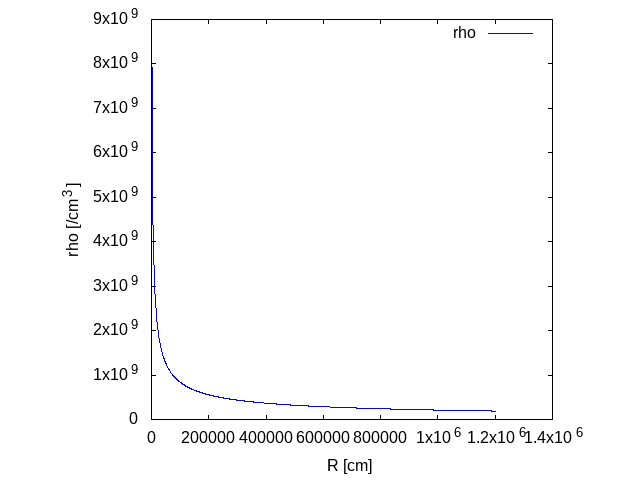
\includegraphics[scale=0.45]{pro1a.png}
        \label{fig:pro1a}
    }
    \subfigure[another case of trying]{
        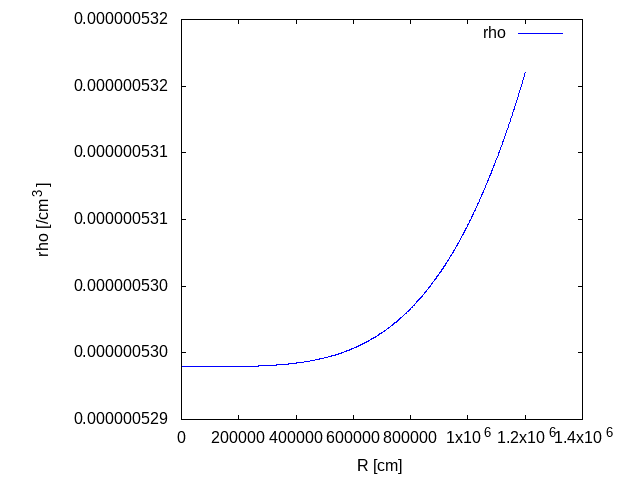
\includegraphics[scale=0.45]{pro1b.png}
        \label{fig:pro1b} 
    }
    \caption{case of trying}
    \label{fig:pro1}
\end{figure}
% %-------------------------------

\subsubsection*{Q1.b. : mass with radius}
Because I stuck in question 1, so didn't accomplish this part.




\begin{thebibliography}{00}

\bibitem{b1}
Sun Fact Sheet from NASA\\
 \href{(https://nssdc.gsfc.nasa.gov/planetary/factsheet/sunfact.html).}{(https://nssdc.gsfc.nasa.gov/planetary/factsheet/sunfact.html).}

\bibitem{b2}
Calculate the mean molecular weight $\mu$\\
 \href{https://web.njit.edu/~gary/321/Lecture7.html}{https://web.njit.edu/~gary/321/Lecture7.html}
 
\end{thebibliography}

\end{document}

% \footnote{Lagrangian point:\href{https://en.wikipedia.org/wiki/Lagrange\_point}{https://en.wikipedia.org/wiki/Lagrange\_point}}


% %-------------------------------
% \begin{figure}[h]
%     \centering 
% 	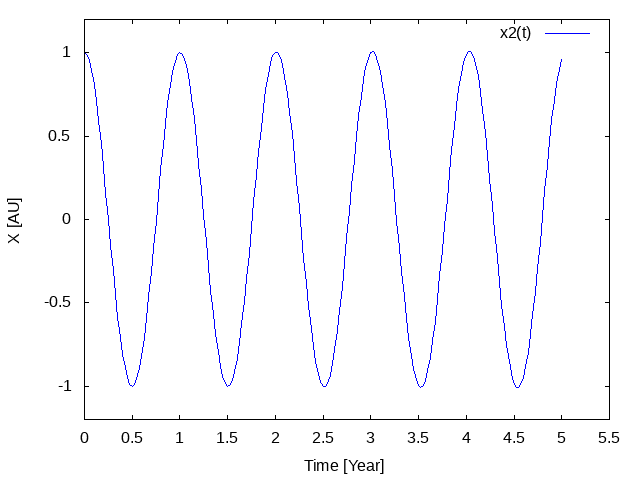
\includegraphics[scale=0.45]{pro1_x2.png}
% 	\caption{The trajectory of $m_1$ $m_2$ (when $m_2$ has a 1.25 factor of velocity).} %圖片註解
% 	\label{fig.pro1} %label 用這個就可以引用文章當中
% \end{figure}
% %-------------------------------

% %-------------------------------
% \begin{figure}[h]
%     \centering
%     \subfigure[dt=0.01yr]{
%         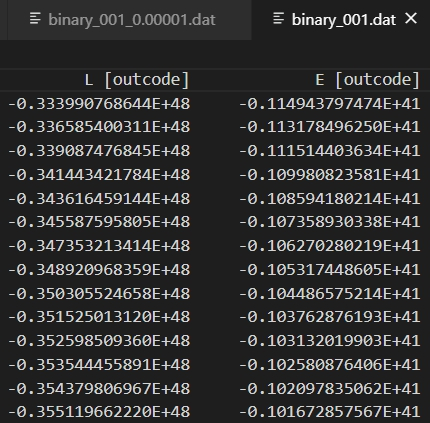
\includegraphics[scale=0.33]{01.jpg}
%         \label{01}
%     }
%     \subfigure[dt=0.001yr]{
%         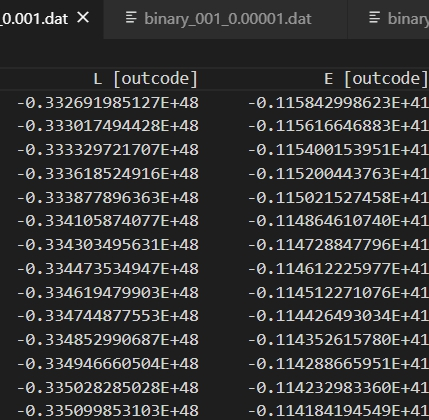
\includegraphics[scale=0.33]{001.jpg}
%         \label{001} 
%     }
%     \subfigure[dt=0.00001yr]{
%         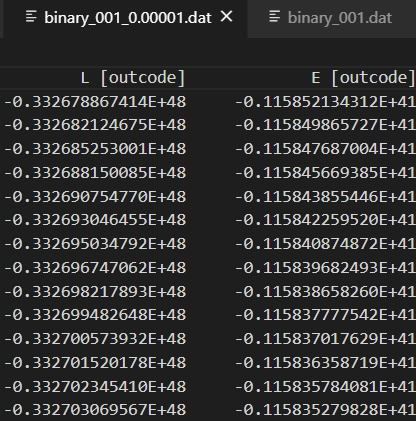
\includegraphics[scale=0.33]{00001.jpg}
%         \label{00001} 
%     }
%     \caption{L \& E in 0.01,0.001,0.00001 time step}
%     \label{fig:2c_dat}
% \end{figure}
% %-------------------------------
